\documentclass{article}


% This file is a solution template for:
% 1 inch margins
\usepackage{fullpage}

\usepackage{booktabs}
\usepackage{longtable}

\usepackage{hyperref}
\usepackage{graphicx}
\usepackage{multicol}
\usepackage{subcaption}

% Add ability to resume enumeration environments with /begin{enumerate}[resume]
\usepackage{enumitem}

\usepackage{pgf}
\usepackage{tikz}
\usepackage{bodegraph}
\usepackage{circuitikz}
\usetikzlibrary{calc}
\usetikzlibrary{trees}
\usetikzlibrary{arrows}
\usetikzlibrary{shapes}
\usetikzlibrary{fadings}
\usetikzlibrary{positioning}
\usetikzlibrary{intersections}


\usepackage[english]{babel}
\usepackage[latin1]{inputenc}
\usepackage[T1]{fontenc}
% Or whatever. Note that the encoding and the font should match. If T1 does not look nice, try deleting the line with the fontenc.


\usepackage{listings}

\usepackage{amsmath}


\usepackage{xspace}
\newcommand{\Ohm}{$\Omega$\xspace}



\title{Electronic Circuit Simulation and Layout Software}


\begin{document}
\maketitle

In this lab we introduce the use of analog circuit simulation software and circuit layout software.

\section{Introduction}
So far we have designed all of our circuits by studying basic electronic subcircuit building blocks and then constructing larger circuits from these. We have designed our circuits by calculating their steady state behavior, as well as their response to small AC (sine wave) signal deviations from the quiescent state. While this method is useful for coming up with the overall design of a circuit, it is a slow and limited method for predicting the ideal theoretical behavior of a circuit under all experimental conditions. 
\subsection{Computer-based analog circuit simulators}
Computer software circuit simulators are very good at calculating ideal theoretical behavior from Kirchhoff's Laws. While circuit simulators will not help you come up with the insight or the creativity to design a good circuit, they are very useful for helping to elucidate quickly the benefits and disadvantages of one circuit design against another. Generally, you can simulate a circuit much more quickly than you can build and test it on a breadboard (after a little practice, of course). The circuit simulator also allows you to try out many variations on a circuit relatively quickly.

The industry standard analog circuit simulation software is SPICE (Simulation Program with Integrated Circuit Emphasis), which was originally developed at UC Berkeley during the 1970's and early 1980's. SPICE (v2G.6) is the basis for many commercial computer software programs. These programs provide the GUI (Graphical User Interface), but use the SPICE (or WinSPICE) simulation engine to perform all the circuit calculations.

SPICE does not simulate the electromagnetic fields in a circuit since these depend explicitly on the layout of the circuit. The results of SPICE can be trusted up to the low MHz range, but should be treated with suspicion for higher frequencies.

In this course, we will use the commercial software 5Spice (free for non-commercial use, avialable for Mac and Windows) available from \url{http://www.5spice.com}.

\subsection{Computer-based circuit layout editor}
In the electronics labs, you have designed the layout of your breadboard circuits on the fly. In a professional setting, the layout of a circuit determines its compactness, ease of use (and debugging), cost, longevity, and its performance (especially at high frequencies). A number of programs exist to help with circuit layout. In fact in industry, most electronics engineers will design an abstract circuit with a circuit simulator and then use a software package to layout the actual circuit on a PCB (Printed Circuit Board). The PCB layout design is then turned into an industry standard Gerber file which is sent to a PCB production company. A prototype will be assembled and tested at the engineering company from a PCB board and electronics components, and once it is tested the entire production is usually contracted out to a third company.

In a physics research lab, the production is done in house, generally. The use of professionally made PCBs is relatively common, since it generally results in a reproducible circuit, which is likely to work better at high frequencies than one put together with wires or prototyping boards.

In this course, we will use the commercial software EAGLE by CadSoft (free for non-commercial use) available from \url{http://www.cadsoftusa.com}.

\section{5Spice}
Circuit simulation is a two step process. In the first step you must construct the actual circuit diagram using wires and electronics components (i.e. resistor, capacitors, inductor, diodes, integrated circuits, etc,\ldots). In the second step, you vary the inputs to your circuit and see how it affects the circuit operation and the outputs.

The simplest way to introduce 5Spice is with an example, so we will make and analyze a low-pass $RC$ filter, as shown in Figure~\ref{fig:rc_low_pass_filter}.  It is not important to fully understand the circuit right now; we just use it as a reasonably complete example with which we can demonstrate the work flow.  Tutorial videos are also available online, in the YouTube channel \href{https://www.youtube.com/channel/UCC1qbSb4QSiS_0mZziTIxTA}{5SpiceOfficial}.

\begin{figure}
 \begin{center}
  \begin{circuitikz}
   \draw (-2,2) node[left]{$v_{in}$} to[R,l=10\,k\Ohm,o-] (0,2) to[C,l=10\,nF] (0,0) node[ground]{};
   \draw (0,2) to[short,-o] (1,2) node[right]{$v_{out}$};
  \end{circuitikz}
  \caption{The $RC$ filter circuit that we will implement in 5Spice.  The cut-off frequency is $\omega = 1/RC = 10$\,kHz.}
  \label{fig:rc_low_pass_filter}
 \end{center}
\end{figure}

The program is relatively easy to use. When you start the program you will get a blank schematic drawing canvas. The important GUI elements (i.e. the ones you will use the most) of the main screen are shown in Figure~\ref{fig:5spice:startup_screen}.

\begin{figure}
\begin{center}
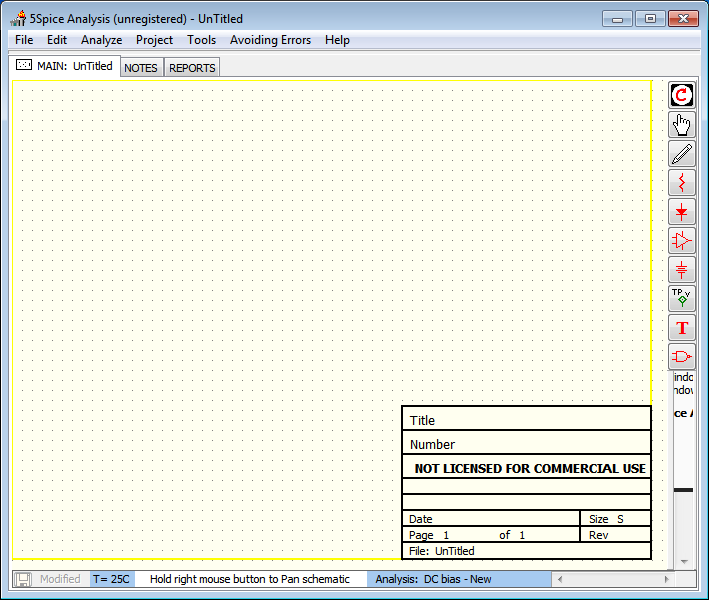
\includegraphics[width=0.6\textwidth]{pics/5spice_startup_screen}
\end{center}
\caption{The 5Spice start screen has a toolbox bar with frequently used icons on the right.  From top to bottom they are: run calculation, cursor mode, wires, passive elements (resistors, capacitors, inductors), semiconductor elements, ICs and active components, voltage and current sources, test points, text, and logic gates.}
\label{fig:5spice:startup_screen}
\end{figure}

\subsection{Circuit diagram}
The first step is to build the circuit diagram of Figure~\ref{fig:rc_low_pass_filter}.

We start with the passive components: the resistor and the capacitor. We insert the capacitor by going to the passive components menu (the resistor icon) on the toolbox bar and selecting the resistor sub-element which we then drop onto the schematic canvas as shown in Figure~\ref{fig:5spice:add_component}.

\begin{figure}
\begin{center}
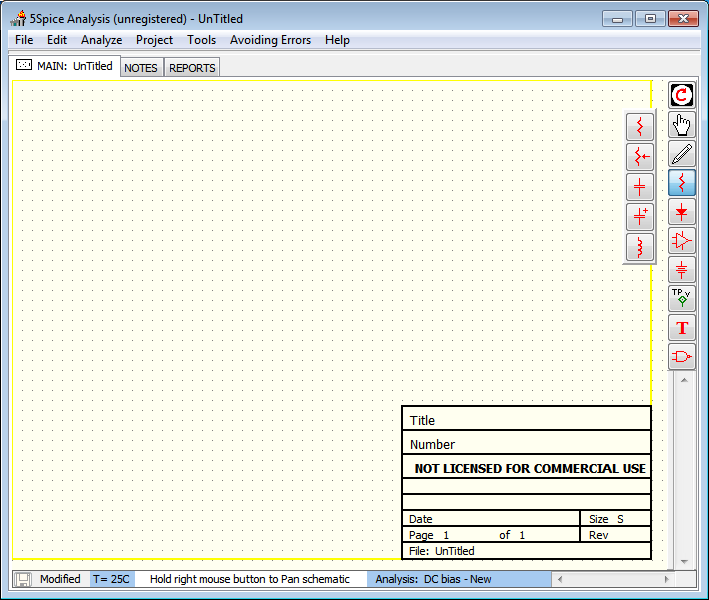
\includegraphics[width=0.6\textwidth]{pics/5spice_add_component}
\end{center}
\caption{We select the capacitor and drop it onto the schematic canvas.}
\label{fig:5spice:add_component}
\end{figure}

The schematic canvas now has a single capacitor in the middle of it. Figure~\ref{fig:5spice:component_dropped} shows the schematic with a single capacitor with a default value of 10\,nF.

\begin{figure}
\begin{center}
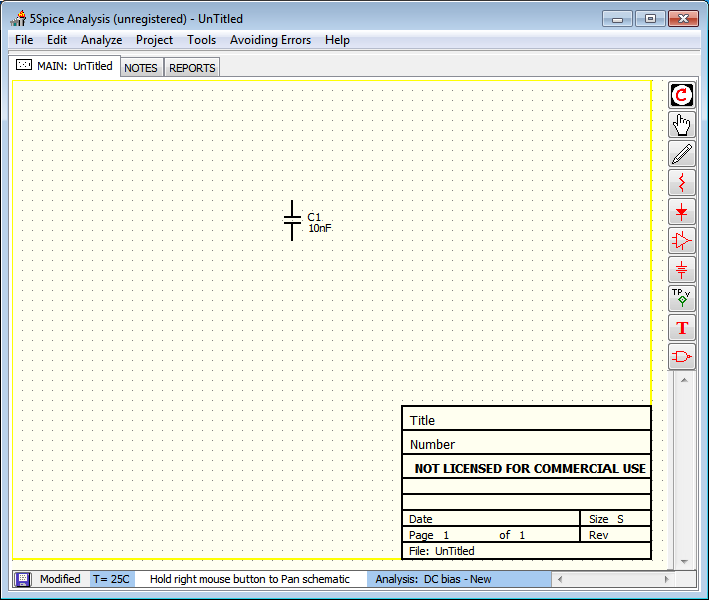
\includegraphics[width=0.6\textwidth]{pics/5spice_component_dropped}
\end{center}
\caption{The schematic canvas now contains a single capacitor with a default value of 10\,nF.}
\label{fig:5spice:component_dropped}
\end{figure}

We can change the value of the capacitance by selecting the component, right-clicking on the component, and selecting the ``Edit Parameter'' menu listing.  For the capacitor this brings up the dialog shown in Figure~\ref{fig:5spice:edit_parameter} where we can set the value for the capacitance.  For more complicated components, e.g. diodes, the ``Edit Parameter'' selection calls up the sub-circuit library, where you can search and choose the desired component model.  If you cannot find the SPICE model for the component that you are looking for in the library, you can generally find it on the manufacturer's website. If not then you must simulate with another component.

\begin{figure}
\begin{center}
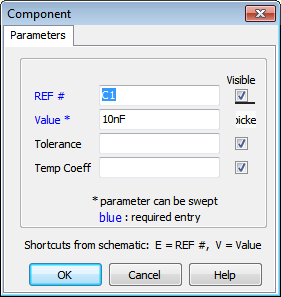
\includegraphics[width=0.3\textwidth]{pics/5spice_edit_parameters}
\end{center}
\caption{The ``Edit Parameter'' dialog allows to change the capacitance value.}
\label{fig:5spice:edit_parameter}
\end{figure}

We must now construct the rest of the circuit.  We add the resistor from the passive components icon menu on the right, using the select-and-drop technique.  When we put the resistor on the schematic canvas, it is vertical.  We rotate it by right-clicking on the resistor component image and selecting the ``rotate'' menu listing.  Also the resistor can be left at its default value of 10\,k\Ohm.

We are now ready to add the reference ground to our circuit (without this the simulation will not be possible).  We do this with ``power'' toolbox menu.  We select-and-drop the ground to its desired location.

The last additions to the circuit diagram are the input and output signals: we add a voltage signal source for the input and a ``voltage test point'' for the output.

We only need to add the wires in to make our low-pass $RC$ filter.  We do this by selecting the ``wire'' from the wire drawing icon menu, as shown in Figure~\ref{fig:5spice:adding_wires}.  We draw in the wires for the low-pass $RC$ filter using the mouse cursor.  You can stop a wire trace by hitting the ``esc'' (escape) key.

\begin{figure}
\begin{center}
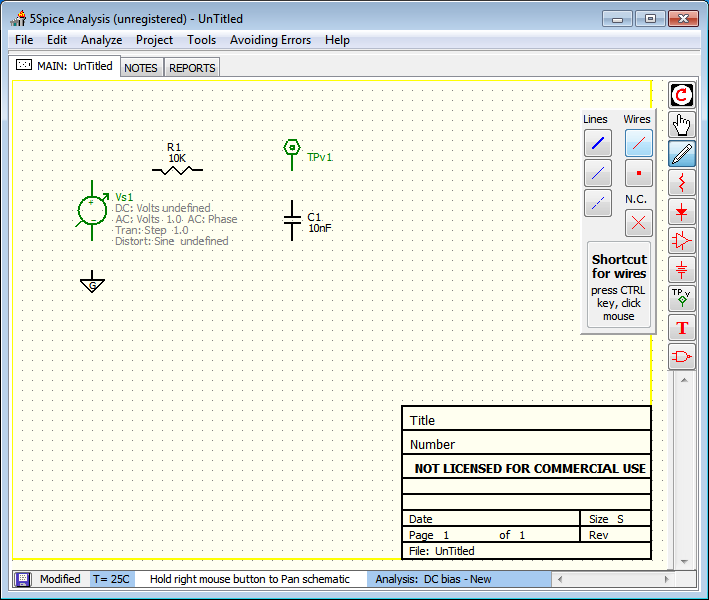
\includegraphics[width=0.6\textwidth]{pics/5spice_adding_wires}
\end{center}
\caption{We select the wire drawing tool to add the wire connections.  Notice that proper wire junctions are indicated with a small filled circle.}
\label{fig:5spice:adding_wires}
\end{figure}

The completed circuit, with all components connected by wires, is shown in Figure~\ref{fig:5spice:added_wires}.

\begin{figure}
\begin{center}
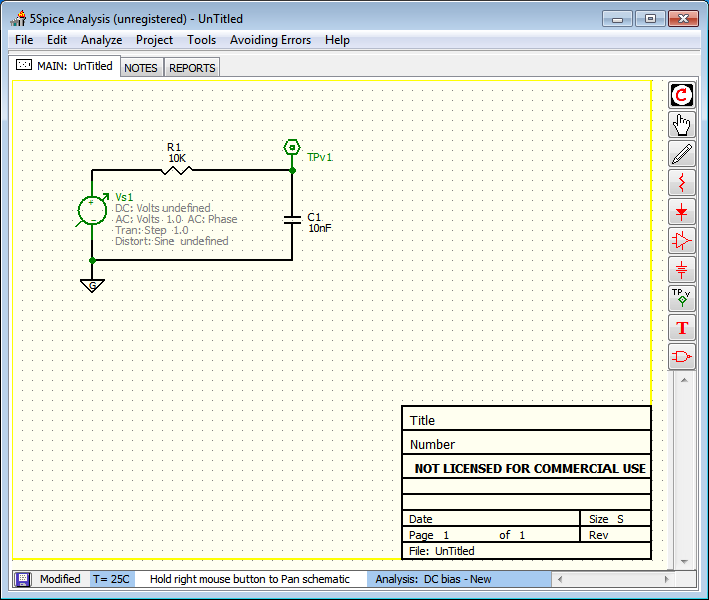
\includegraphics[width=0.6\textwidth]{pics/5spice_added_wires}
\end{center}
\caption{The completed circuit, after adding all components and all wires, is now ready for simulations.}
\label{fig:5spice:added_wires}
\end{figure}


\subsection{Circuit analysis}
We are now ready to analyze the ideal theoretical performance of our low-pass $RC$ filter circuit. All circuit analysis starts with the ``analysis dialog'' which you can access through the ``Analyze'' menu.

The ``analysis dialog'' allows you to perform three principal types of analysis on the a circuit: i) ``DC bias'', ii) ``AC'', and iii) ``Transient''. The analysis type can be chosen in the  ``analysis'' tab of the ``analysis dialog'' as shown in Figure~\ref{fig:5spice:select_analysis}.

\begin{figure}
\begin{center}
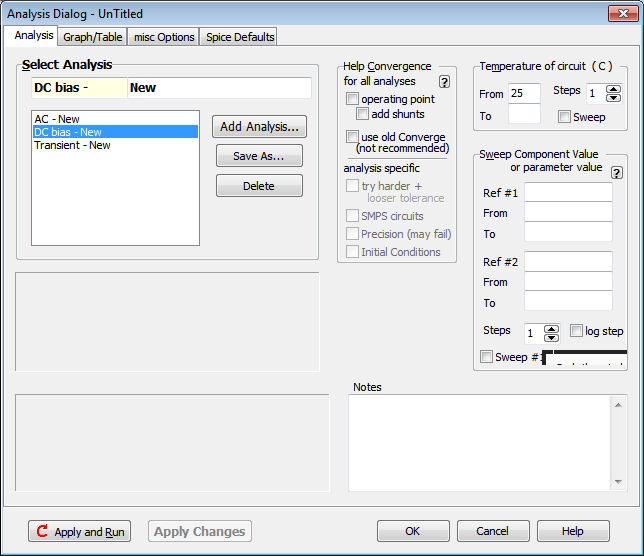
\includegraphics[width=0.6\textwidth]{pics/5spice_select_analysis}
\end{center}
\caption{The analysis dialog is used to select the type of analysis to be performed.}
\label{fig:5spice:select_analysis}
\end{figure}

\subsubsection{DC bias analysis}
You use this analysis to determine the steady-state or quiescent operation of a circuit. This type of analysis does not produce a plot. When we apply it to our $RC$ filter circuit by clicking the ``Apply and Run'' button, 5Spice calculates the DC voltages and currents and sends the output to the new ``DC Bias'' tab of the main window as shown in Figure~\ref{fig:5spice:DC_bias}.  In our case, without addition of a bias voltage at the input source, the bias voltages are all zero.

\begin{figure}
\begin{center}
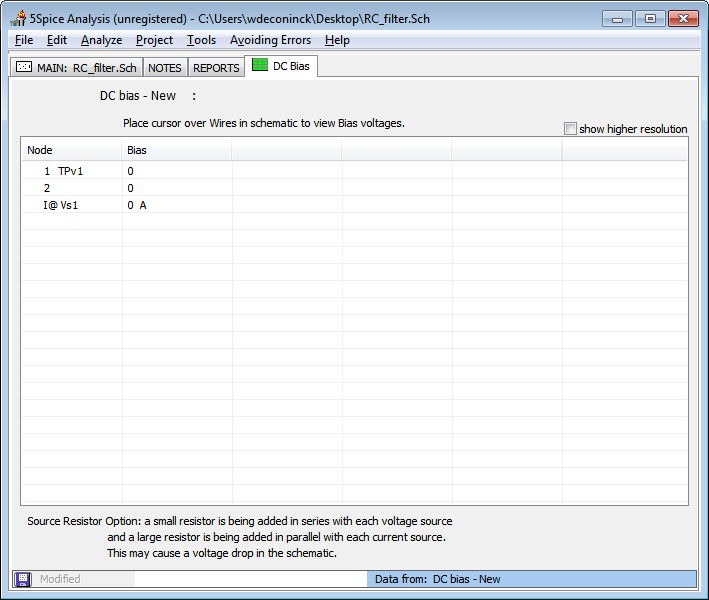
\includegraphics[width=0.6\textwidth]{pics/5spice_DC_bias}
\end{center}
\caption{The results of the ``DC bias'' analysis can be found in the ``DC Bias'' tab of the main window.}
\label{fig:5spice:DC_bias}
\end{figure}

\subsubsection{AC analysis}
We use the ``analysis dialog'' to setup an AC analysis as shown in Figure~\ref{fig:5spice:AC_analysis}. The AC analysis consists of sending an AC signal into the input, determined by the voltage signal source in the circuit diagram, and scanning the frequency to determine the frequency response of the circuit output or at any other test point. In our case, we scan the frequency of the input from 10\,Hz to 1\,MHz. The AC analysis is done in frequency space (i.e. Fourier space).

\begin{figure}
\begin{center}
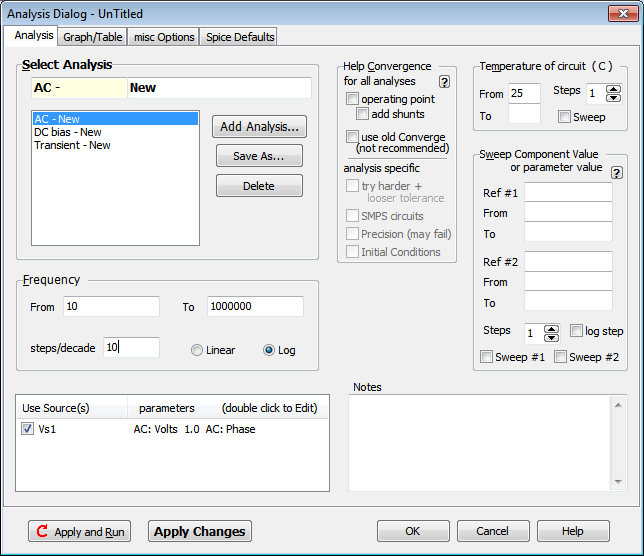
\includegraphics[width=0.6\textwidth]{pics/5spice_AC_analysis}
\end{center}
\caption{The AC analysis setup is more involved than the DC bias analysis.}
\label{fig:5spice:AC_analysis}
\end{figure}

The AC analysis generally outputs a Bode plot of the frequency scan. The plot can be tailored to the circuit and the analysis in the ``Graph/Table'' tab of the ``Analysis Dialog'' as shown in Figure~\ref{fig:5spice:AC_analysis_output_graphs}. For our AC analysis we choose to plot both the magnitude and phase of the output AC signal.

\begin{figure}
\begin{center}
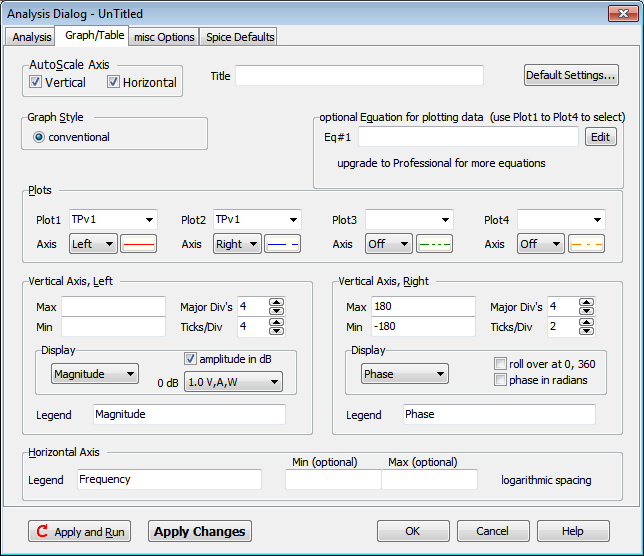
\includegraphics[width=0.6\textwidth]{pics/5spice_AC_analysis_output_graphs}
\end{center}
\caption{The ``Graph/Table'' tab allows us to define the output graphs for the AC analysis.  Notice the vertical and horizontal autoscale check boxes in the top right.}
\label{fig:5spice:AC_analysis_output_graphs}
\end{figure}

When we run the AC analysis, 5Spice calculates the behavior of the output over the entire frequency scan, and produces the output Bode plots shown in Figure~\ref{fig:5spice:AC_analysis_results}. The graphs are displayed in the ``AC-1'' tab of the 5Spice main window.

\begin{figure}
\begin{center}
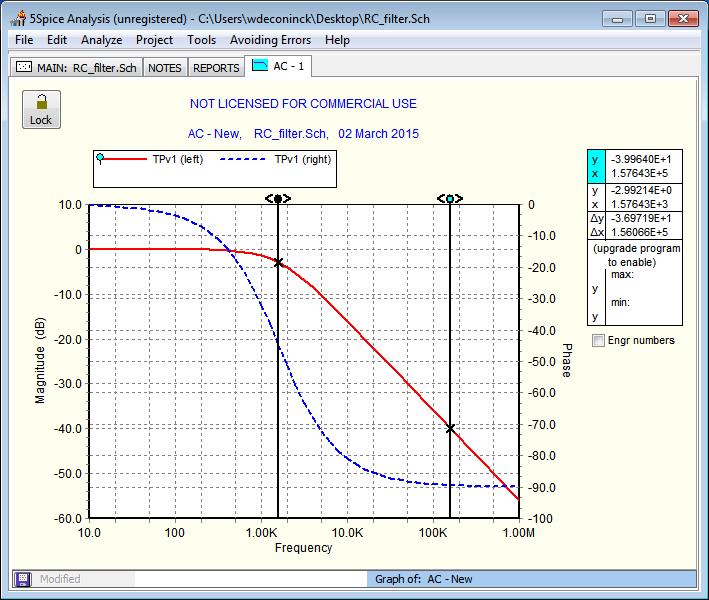
\includegraphics[width=0.6\textwidth]{pics/5spice_AC_analysis_results}
\end{center}
\caption{The AC analysis output plots show both the magnitude and the phase of the output signal at the test point. The graph also features two sliding readouts, which are here set to the 3\,dB frequency and to a frequency 100 times larger.}
\label{fig:5spice:AC_analysis_results}
\end{figure}

If necessary the computed values used for the plots can be saved to a file---they are also displayed in the ``Reports'' tab of the main 5Spice window.

\subsubsection{Transient analysis}
Transient analysis is done in the time domain. SPICE numerically computes the time evolution of the circuit voltages and currents as function of some time-varying input. The transient analysis is set to compute the time evolution from $t = 0$\,s to $t = 0.0002$\,s, as shown in Figure~\ref{fig:5spice:transient_analysis}.  For our transient analysis, we choose to use a 10\,kHz square wave with 0.1\,V DC offset and 0.2\,V pk-pk, which we have selected in the ``Analysis'' tab of the ``Analysis Dialog'' window, as shown in Figure~\ref{fig:5spice:transient_analysis_square_wave}. 

\begin{figure}
\begin{center}
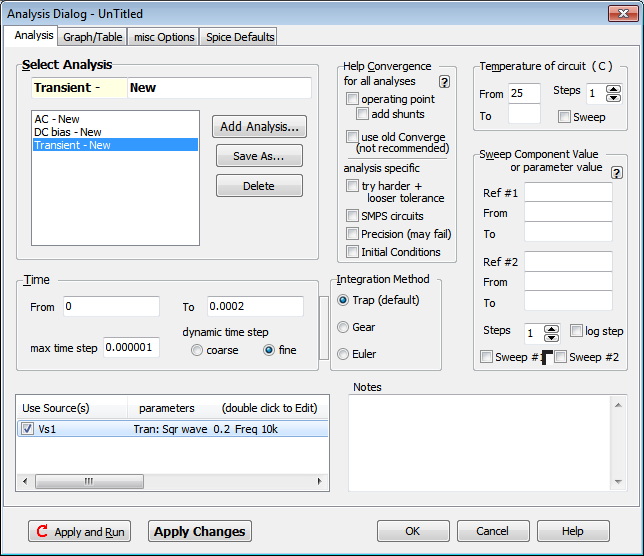
\includegraphics[width=0.6\textwidth]{pics/5spice_transient_analysis}
\end{center}
\caption{The transient analysis is selected and a simulation time is specified.}
\label{fig:5spice:transient_analysis}
\end{figure}

\begin{figure}
\begin{center}
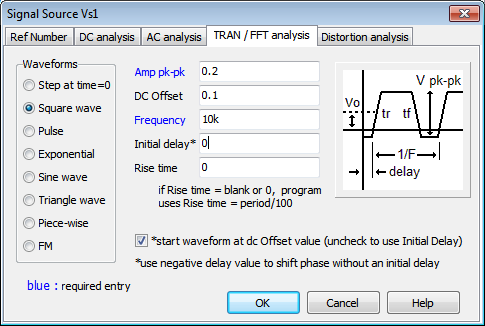
\includegraphics[width=0.6\textwidth]{pics/5spice_transient_analysis_square_wave}
\end{center}
\caption{Double-clicking the source parameters bring up the square wave input parameter dialog.}
\label{fig:5spice:transient_analysis_square_wave}
\end{figure}

Transient analysis is the most difficult and frequently one must adjust the parameters governing the numerical computation in order for the simulation to work. Some of the check boxes in Figure~\ref{fig:5spice:transient_analysis} can help the transient analysis to converge.

If the transient analysis cannot produce a solution even after adjusting the above selections, then the parameters governing the tolerances and convergence criterion for the numerical computation must be modified.  Figure~\ref{fig:5spice:numerical_tolerances} shows the ``Spice Defaults'' tab and dialog in the ``Analysis Dialog'' window. The various parameters should be adjusted to obtain a transient numerical solution, though care must be taken since these adjustments will also affect the accuracy of the analysis results.  

\begin{figure}
\begin{center}
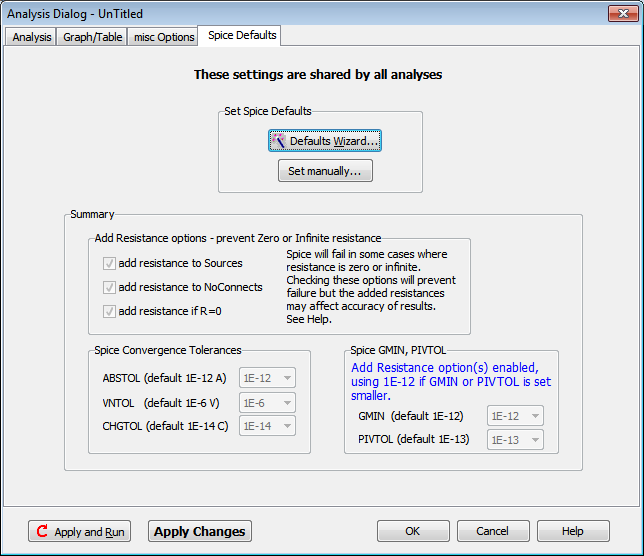
\includegraphics[width=0.6\textwidth]{pics/5spice_numerical_tolerances}
\end{center}
\caption{The numerical computation convergence tolerances and additional parameters can be modified in the ``Spice Defaults'' tab.}
\label{fig:5spice:numerical_tolerances}
\end{figure}

The results of the transient analysis are plotted versus time. The graphs must be setup in a similar manner as shown in Figure~\ref{fig:5spice:AC_analysis_output_graphs} for the AC analysis.  The output is plotted in the ``Transient-1'' tab of the main 5Spice window. As Figure~\ref{fig:5spice:transient_results} shows, our low-pass $RC$ filter acts indeed as an integrator, though it does show some distortion away pure integration of the square input signal due to the exponential behavior of the charging capacitor. If we were to make the actual circuit in the lab, we should not expect better performance than what is shown in Figure~\ref{fig:5spice:transient_results}.

\begin{figure}
\begin{center}
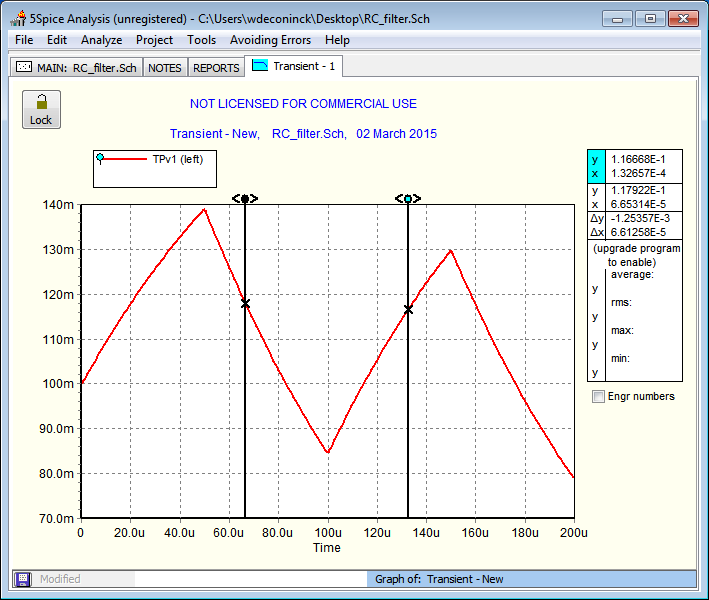
\includegraphics[width=0.6\textwidth]{pics/5spice_transient_results}
\end{center}
\caption{The plot of the transient analysis results for the low-pass $RC$ filter with a square wave input signal shows that the low-pass $RC$ filter acts as an integrator.}
\label{fig:5spice:transient_results}
\end{figure}

In conclusion, we have shown how to construct a circuit diagram with 5Spice and do DC bias, AC, and transient analysis of a circuit. This introduction is not meant to be comprehensive and the reader is encouraged to read up further on how to use 5Spice from the ``help'' menu, or consult the more advanced tutorial videos in the YouTube channel \href{https://www.youtube.com/channel/UCC1qbSb4QSiS_0mZziTIxTA}{5SpiceOfficial}.


\section{EAGLE}
EAGLE is circuit layout software. It is used for converting a circuit diagram into a circuit layout which can be sent to printed circuit board manufacturer for automated production.

As with 5Spice, you must first make a circuit diagram so that EAGLE can help produce a circuit layout. This is a two step process, and we will go through it by using the example of the $RC$ filter of the previous section, but we added a second stage to make it a band-pass filter to fill up the board a bit more (with fewer components the topology does not require two layers).

For additional information on using EAGLE, there are some good tutorials available.  In particular the following series of SparkFun tutorials is recommended:
\begin{itemize}
\item \href{https://learn.sparkfun.com/tutorials/how-to-install-and-setup-eagle}{How to install and setup EAGLE},
\item \href{https://learn.sparkfun.com/tutorials/using-eagle-schematic}{Using EAGLE: Schematic},
\item \href{https://learn.sparkfun.com/tutorials/using-eagle-board-layout}{Using EAGLE: Board Layout}
\end{itemize}

\subsection{Circuit design}
Circuit design in EAGLE is similar to 5Spice. You open a blank schematic canvas, as shown in Figure~\ref{fig:eagle:schematic_blank}, and drag-and-drop components from a library onto it. You then attach the components with wires and add input and output. You must select the ``Use'' menu item in the ``Library'' menu of an EAGLE schematic window to open up a library and access its components (manufacturers may supply libraries with their components, but EAGLE comes with a large selection of components as well).

\begin{figure}
\begin{center}
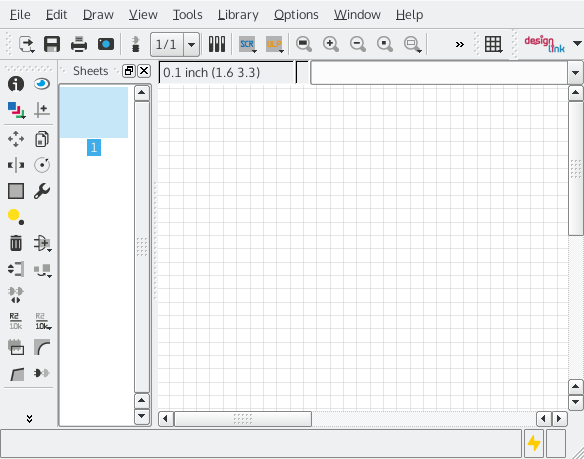
\includegraphics[width=0.6\textwidth]{pics/eagle_schematic_blank}
\end{center}
\caption{The blank EAGLE schematic window.}
\label{fig:eagle:schematic_blank}
\end{figure}

To add components, select ``Edit,'' then ``Add\ldots''' (or the corresponding icon on the toolbox bar on the left).  The ``Add'' dialog will pop up with the entire library of components you can choose from.  Since the routing of the traces on the printed circuit board requires information about the size of the components, it is important to choose the correct component packages from the library.

Resistors can be found in the library ``rcl'' and both US \begin{circuitikz} \ctikzset{bipoles/length=.6cm} \draw (0,0) to [american resistor] (1,0); \end{circuitikz} and European \begin{circuitikz} \ctikzset{bipoles/length=.6cm} \draw (0,0) to [european resistor] (1,0); \end{circuitikz} symbols are available, with no difference in the actual component.  The package size indication (e.g. 0207/10) uses the format \texttt{WWLL/SS} where \texttt{WW} is the body width, \texttt{LL} is the body length, and \texttt{SS} is the hole spacing, all in truncated millimeters.  For example, a standard $1/4$\,W resistor has a diameter of 2.5\,mm (truncate to \texttt{02}), a length of 7\,mm (\texttt{07}), and can be soldered in holes that are 10\,mm apart (\texttt{10}).  Therefore, a resistor R-US\_0207/10 would be a good choice.  If you place the same resistor vertically, R-US\_0207/2V would be a good choice.  As indication of the size of components, a typical breadboard hole spacing is $1/10$ inch.

Capacitors can also be found in the library ``rcl'' but are not as easy to classify by size.  There are again  US \begin{circuitikz} \ctikzset{bipoles/length=.6cm} \draw (0,0) to [polar capacitor] (1,0); \end{circuitikz} and European \begin{circuitikz} \ctikzset{bipoles/length=.6cm} \draw (0,0) to [capacitor] (1,0); \end{circuitikz} symbols, with no difference in the actual component.  The package size indication now uses the format \texttt{SSS-WWWxLLL}, where \texttt{SSS} is the lead spacing (now in units of tenths of a mm, so a typical 5\,mm spacing results in \texttt{050}), \texttt{WWW} is the body width, and \texttt{LLL} is the body length.  Since the lead spacing is the most important parameter, it does not really matter what the other parameters.  A good choice for flat capacitors is \texttt{050-025x075}.  You will find polarized capacitors (which are typically round) under the name ``CPOL,'' this time with designations such as \texttt{E5-8.5} for an electrolytic (\texttt{E}, as opposed to \texttt{TT} for tantalum) capacitor with 5\,mm lead spacing and a diameter of 8.5\,mm.

Finally, we need an input port and output port for our filter.  We can choose a right-angle BNC coaxial connector for both in and output, and we wire everything together with the ``Net'' tool to create an electrical connection (``Wire'' just draws a line and is unfortunately a confusingly names decoy here).  As an example, Figure~\ref{fig:eagle:schematic_bandpass} shows the EAGLE schematic window with a band-pass double $RC$ filter connected to BNC coaxial connectors for both input and output.

\begin{figure}
\begin{center}
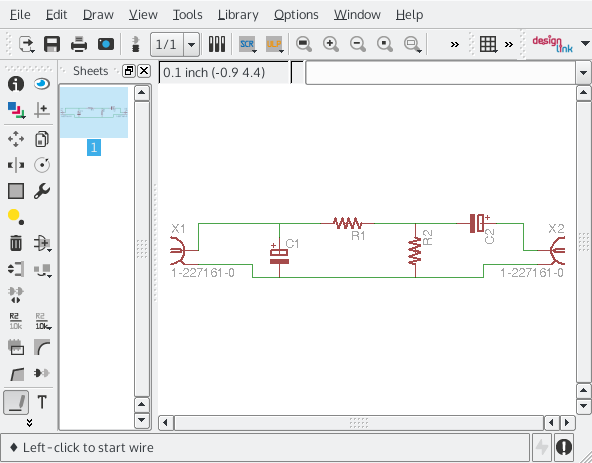
\includegraphics[width=0.6\textwidth]{pics/eagle_schematic_bandpass}
\end{center}
\caption{The EAGLE schematic window.}
\label{fig:eagle:schematic_bandpass}
\end{figure}

\subsection{Circuit layout}
Once the schematic is complete, it can be converted to a board by selecting the ``File'' -- ``Switch to board'' menu command, or the corresponding icon button.  

\begin{figure}
\begin{center}
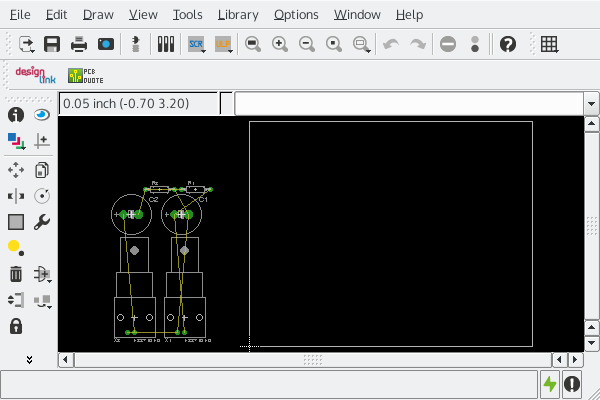
\includegraphics[width=0.6\textwidth]{pics/eagle_board_start}
\end{center}
\caption{The ``Switch to board'' menu or button generates an initial board from the schematic, but you are responsible for placing the components and drawing the traces.}
\label{fig:eagle:board_start}
\end{figure}

The printed circuit board produced with ``Switch to board'' menu or button still requires a lot of work. The first step is to place all the components appropriately into the board area as indicated in Figure~\ref{fig:eagle:board_start}.  

An important fact to remember is that the board has two sides which you can use for placing components and routing wires/traces. The next step is to route all the wires. This can be done to a certain extent with the ``Autorouter'' feature, though one must still route some of the wires by hand, generally. The wire routing is shown in Figure~\ref{fig:eagle:board_autorouter} below.

\begin{figure}
\begin{center}
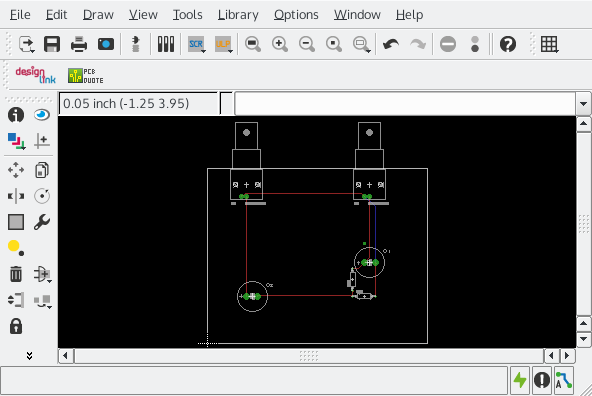
\includegraphics[width=0.6\textwidth]{pics/eagle_board_autorouter}
\end{center}
\caption{The ``Autorouter'' does an acceptable job for simple circuits.}
\label{fig:eagle:board_autorouter}
\end{figure}

The wire routing is generally the bulk of the work and can take quite a long time. You should remember that the circuit is really 3-dimensionall and that one can use a holes and vias (conducting hole) to connect components and wires.

When making a board that will work at RF frequencies, a good rule of thumb is to have as much metal around which is at a ground voltage. These large areas of metal are called ``ground planes'' and help shield parts of the circuit from one another. Furthermore, one should try to make sure that all the wires are also transmission lines (ideally with 50\,\Ohm RF impedance), so that each wire has a ground on either side of it (and above or below it, depending on the orientation).  Figure~\ref{fig:eagle:board_complete} shows the board after filling in all the blank areas with ground planes.

\begin{figure}
\begin{center}
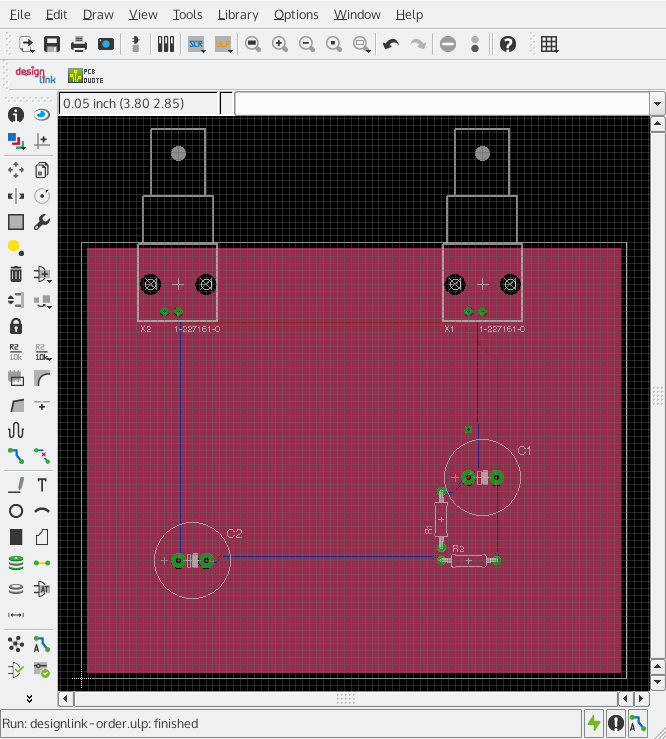
\includegraphics[width=0.6\textwidth]{pics/eagle_board_complete}
\end{center}
\caption{Finished board with ground planes and holes for components. All the ground wires have been replaced by ground planes.}
\label{fig:eagle:board_complete}
\end{figure}

\subsection{The Gerber file}
The Gerber file is an industry standard computer file which contains all the information necessary for making a PCB (Printed Circuit Board). Once your board is finished, you can make a Gerber file by going to the CAM window under ``File'' -- ``CAM Processor''. Once in the CAM window select the device to be ``GERBERAUTO'' and include a filename. The ``process job'' button will produce a set of Gerber files which you can send to a PCB manufacturer for automated production (for example \href{http://oshpark.com/}{OSH Park} or \href{http://www.4pcb.com/}{Advanced Circuits}).

The CAM processor also has ``EPS'' and ``PS'' devices which will create accurate images for DIY PCB printing.  The resulting files are shown in Figure~\ref{fig:eagle:board_eps}.  

\begin{figure}
\begin{center}
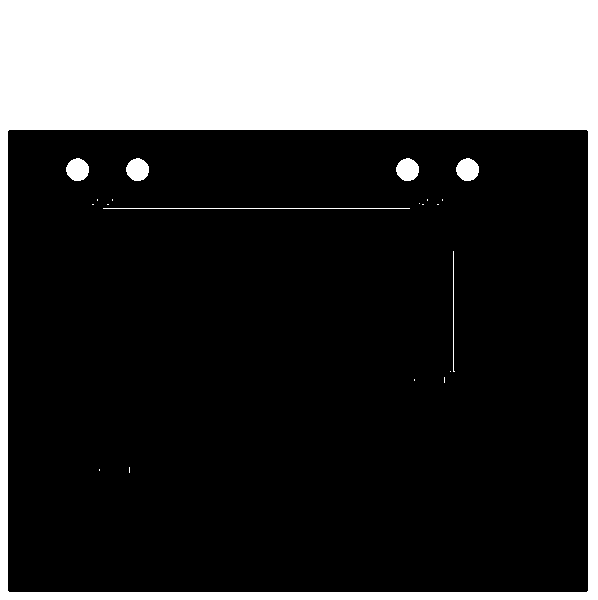
\includegraphics[width=0.45\textwidth]{pics/band_pass_bottom} 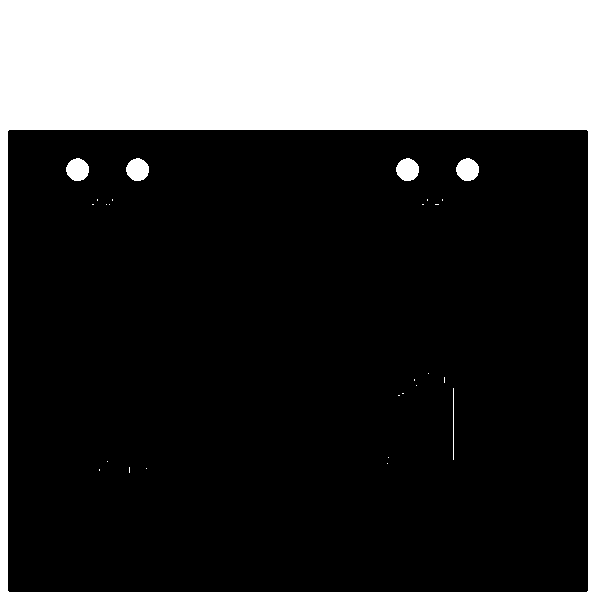
\includegraphics[width=0.45\textwidth]{pics/band_pass_top}
\end{center}
\caption{Output EPS files as produced by the CAM processor in EAGLE.}
\label{fig:eagle:board_eps}
\end{figure}

In conclusion, we have shown how to construct a circuit diagram and PCB with EAGLE. This introduction is not at all comprehensive and the reader is encouraged to find further information on how to use EAGLE from the ``help'' menu.

\pagebreak

\section{Lab 6: Electronic Circuit Simulation and Layout Software}
This week's lab focuses on the use of the 5Spice analog circuit simulator and the EAGLE printed circuit board layout software.

\begin{enumerate}
\item Use the 5Spice circuit simulator to determine the $IV$ curve of the diodes 1N4007 and 1N4148 between -2\,V and +2\,V.  Since the free version of 5Spice does not allow you to create $x$ vs. $y$ graphs, you will need to sweep the DC voltage of the signal voltage source and measure the current through the diode without having a resistor connected in series (contrary to what we did in real life).

\item Use the 5Spice circuit simulator to simulate the behavior of the full-wave rectifier circuit in the previous lab.  Use as diode the model 1N4148, and use the transformer model ``Pi'' with Ls1 = 0, Lm = 0.1, and N = 5.  Include the measured values for the primary and secondary coils of the transformer as Rs1 and Rs2.  Place a 50\,\Ohm resistor in series with the input voltage source to simulate the output impedance of the signal generator.
\begin{enumerate}
\item Use the transient analysis tool to determine the response of the circuit without buffering capacitor to a sine-wave input voltage with a zero DC offset voltage, an amplitude of 1\,V, and a frequency of 1\,kHz.  Use a 100\,k\Ohm resistor as load.  \emph{Hint:} Try to look at a transient analysis time window that spans about 10 periods.
\item Use the transient analysis tool to the find optimal value of the buffering capacitor, such that the ripples are below 10\% of the average output voltage (sweep the value of filtering capacitor in progressively smaller ranges starting with 1\,nF to 1\,$\mu$F).  You will need to look at times sufficiently beyond the start time $t = 0$, but with step sizes that are small compared to the period of the input voltage.
\end{enumerate}

\item Develop a printed circuit board that takes as input (through a BNC connector) an AC signal, sends the signal through an audio transformer (SP-67, similar but not identical to the SP-33 and SP-11 transformers we used in the previous lab, use the outermost terminals for this transformer), and rectifies and filters it before returning a DC signal on another BNC connector.  Generate encapsulated postscript (EPS) masks for the top and bottom layers of your PCB to paste in your lab book (you can convert the EPS files to PDF with graphics software or with online services).
\end{enumerate}

\end{document}
